\documentclass[11pt,a4paper]{article}
\usepackage[spanish,es-nodecimaldot]{babel}	% Utilizar español
\usepackage[utf8]{inputenc}					% Caracteres UTF-8
\usepackage{graphicx}						% Imagenes

\PassOptionsToPackage{hyphens}{url}
\usepackage[hidelinks]{hyperref}			% Poner enlaces sin marcarlos en rojo

\usepackage{fancyhdr}						% Modificar encabezados y pies de pagina
\usepackage{float}							% Insertar figuras
\usepackage[textwidth=390pt]{geometry}		% Anchura de la pagina
\usepackage[nottoc]{tocbibind}				% Referencias (no incluir num pagina indice en Indice)
\usepackage{enumitem}						% Permitir enumerate con distintos simbolos
\usepackage[T1]{fontenc}					% Usar textsc en sections
\usepackage{amsmath}						% Símbolos matemáticos
\usepackage{listings}
\usepackage{algorithm}

\usepackage{color}
 
\definecolor{codegreen}{rgb}{0,0.6,0}
\definecolor{codegray}{rgb}{0.5,0.5,0.5}
\definecolor{codepurple}{rgb}{0.58,0,0.82}
\definecolor{backcolour}{rgb}{0.95,0.95,0.92}
 
\lstdefinestyle{mystyle}{
    backgroundcolor=\color{backcolour},   
    commentstyle=\color{codegreen},
    keywordstyle=\color{magenta},
    numberstyle=\tiny\color{codegray},
    stringstyle=\color{codepurple},
    basicstyle=\footnotesize,
    breakatwhitespace=false,         
    breaklines=true,                 
    captionpos=b,                    
    keepspaces=true,                 
    numbers=left,                    
    numbersep=5pt,                  
    showspaces=false,                
    showstringspaces=false,
    showtabs=false,                  
    tabsize=2
}
 
\lstset{style=mystyle, language=Python}

% Comando para poner el nombre de la asignatura
\newcommand{\asignatura}{Aprendizaje Automático}
\newcommand{\autor}{Vladislav Nikolov Vasilev}

% Configuracion de encabezados y pies de pagina
\pagestyle{fancy}
\lhead{Vladislav Nikolov, José María Sánchez}
\rhead{\asignatura{}}
\lfoot{Grado en Ingeniería Informática}
\cfoot{}
\rfoot{\thepage}
\renewcommand{\headrulewidth}{0.4pt}		% Linea cabeza de pagina
\renewcommand{\footrulewidth}{0.4pt}		% Linea pie de pagina

\begin{document}
\pagenumbering{gobble}

% Pagina de titulo
\begin{titlepage}

\begin{minipage}{\textwidth}

\centering


\includegraphics[scale=0.5]{img/ugr.png}\\

\textsc{\Large \asignatura{}\\[0.2cm]}
\textsc{GRADO EN INGENIERÍA INFORMÁTICA}\\[1cm]

\noindent\rule[-1ex]{\textwidth}{1pt}\\[1.5ex]
\textsc{{\Huge PROYECTO FINAL\\[0.5ex]}}
\textsc{{\Large Subtítulo práctica\\}}
\noindent\rule[-1ex]{\textwidth}{2pt}\\[3.5ex]

\end{minipage}

\vspace{0.5cm}

\begin{minipage}{\textwidth}

\centering

\textbf{Autores}\\ {\autor{}}\\{José María Sánchez Guerrero}\\[2ex]
\textbf{Rama}\\ {Computación y Sistemas Inteligentes}\\[2ex]
\vspace{0.3cm}


\includegraphics[scale=0.3]{img/etsiit.jpeg}

\vspace{0.7cm}
\textsc{Escuela Técnica Superior de Ingenierías Informática y de Telecomunicación}\\
\vspace{1cm}
\textsc{Curso 2018-2019}
\end{minipage}
\end{titlepage}

\pagenumbering{arabic}
\tableofcontents
\thispagestyle{empty}				% No usar estilo en la pagina de indice


\newpage

\setlength{\parskip}{1em}

\section{\textsc{Descripción del problema}}

El conjunto de datos con el que vamos a trabajar es el \textit{Image Segmentation Data Set}, creado por el Vision Group de
la Universidad de Massachusetts. Este conjunto de datos contiene una serie de características de casos extraídos al azar
de una base de datos con 7 tipos de imágenes tomadas al aire libre. Éstas imágenes fueron segmentadas manualmente para
crear una clasificación para cada píxel. Cada instancia es una región de $3 \times 3$.

Originalmente, nuestro conjunto de datos estaba ya dividido en training y test. Sin embargo, disponemos solo de 210 datos
de entrenamiento y 2100 de test. Como la cantidad de datos que tenemos para entrenamiento es muy inferior a la de test, y
no existe un motivo justificado por el que las particiones se hayan hecho de esta forma, hemos decidido juntar todos los
datos y crear nuestras propias particiones de entrenamiento y test. Esta división se comentará con más detalles en
secciones posteriores, cuando hablemos de las transformaciones y preprocesado que hemos realizado sobre los datos de los
que disponemos. 

Según la información proporcionada por la descripción del conjunto de datos, la cuál puede ser encontrada en el
repositorio UCI \cite{bib:uci-repo}, existen 7 clases distintas, y hay 30 muestras de cada clase en el conjunto de
entrenamiento y 300 en el conjunto de test. Con lo cuál, tenemos que en total hay 330 muestras de cada clase si miramos
los dos conjuntos de datos de forma conjunta. En total disponemos de 2310 muestras, cada una de las cuáles tiene 19
atributos que toman valores reales. En la representación original de los datos, tenemos que la primera columna se
corresponde con la clase de la muestra, y las 19 columnas restantes se corresponden con los atributos. 

De esta pequeña descripción podemos concluir que cada clase está idénticamente representada en los datos de los que
disponemos, y que no existe una clase que esté representada en mayor o menor medida que el resto de ellas. 

Con todo esto dicho, vamos a proceder a analizar cada una de las 19 características mencionadas anteriormente, para ver
que representa cada una de ellas:

\begin{enumerate}
	\item \textit{Region-centroid-col}: la columna del píxel central de la región.
	\item \textit{Region-centroid-row}: la fila del píxel central de la región. 
	\item \textit{Region-pixel-count}: el número de píxeles en una región. Su valor siempre es 9. 
	\item \textit{Short-line-density-5}: resultados de un algoritmo de extracción de rectas que cuenta cuántas líneas de longitud 5
	(con cualquier orientación) con bajo contraste, menor o igual a 5, cruzan la región. 
	\item \textit{Short-line-density-2}: igual que \textit{Short-line-density-5} pero cuenta con líneas de alto contraste,
	mayor que 5. 
	\item \label{it:vegde} \textit{Vegde-mean}: mide el contraste de píxeles horizontalmente adyacentes en la región. Hay 6 valores,
	pero se da dan la media y la desviación típica. Este atributo se utiliza como un detector de borde vertical. 
	\item \textit{Vegde-sd:} Desviación típica del contraste de píxeles horizontalmente adyacentes en la región (ver \ref{it:vegde}).
	\item \label{it:hedge} \textit{Hedge-mean}: mide el contraste de los píxeles verticalmente adyacentes.
	Utilizado para la detección de líneas horizontales. Este atributo es el valor medio.
	\item \textit{Hedge-sd}: Desviación típica del contraste de los píxeles verticalmente adyacentes (ver \ref{it:hedge}). 
	\item \textit{Intensity-mean}: el promedio sobre la región de (R + G + B) / 3.
	\item \textit{Rawred-mean}: Promedio sobre la región del valor R. 
	\item \textit{Rawblue-mean}: Promedio sobre la región del valor B. 
	\item \textit{Rawgreen-mean}: Promedio sobre la región del valor G. 
	\item \textit{Exred-mean}: Mide el exceso de rojo: (2R - (G + B)).
	\item \textit{Exblue-mean}: Mide el exceso de azul: (2B - (G + R)).
	\item \textit{Exgreen-mean}: Mide el exceso de verde: (2G - (R + B)).
	\item \label{it:value} \textit{Value-mean}: Transformación 3D no lineal de RGB.
	\item \textit{Saturatoin-mean}: (ver \ref{it:value}).
	\item \textit{Hue-mean}: (ver \ref{it:value}).
\end{enumerate}

Como estamos en un problema de clasificación, cada entrada produce una salida que es una etiqueta. La etiqueta puede hacer
referencia a una de las 7 clases que tiene el problema, las cuáles son: \textit{brickface}, \textit{sky},
\textit{foliage}, \textit{cement}, \textit{window}, \textit{path} y \textit{grass}. Para facilitar la representación de
las clases, vamos a transformar posteriormente cada valor de las etiquetas a un valor numérico. Esto se verá con más
detalle en la siguiente sección, en la que hablaremos del preprocesado realizado sobre los datos.
continuación.

\newpage

\section{\textsc{Preprocesado y transformación de los datos de entrada}}

En esta sección vamos a comentar las transformaciones que hemos realizado sobre los datos originales para adaptarlos

\section{\textsc{Análisis de los datos}}

Para comenzar con el análisis de los datos que tenemos, lo primero tenemos que hacer es, obviamente leer los datos. Para
ello, vamos a comenzar cargándolos en estructuras que nos permita almacenar tanto los datos de entrenamiento como los de
test para posteriormente juntarlos en una única:

\begin{lstlisting}
# Leer los datos de training y test
df1 = read_data_values('datos/segmentation.data')
df2 = read_data_values('datos/segmentation.test')

# Juntar los dos conjuntos en uno solo
df = pd.concat([df1,df2])
\end{lstlisting}

Con los datos ya cargados, nos interesa
Posteriormente, tal y como dijimos en la sección anterior, vamos a juntar los datos en un solo conjunto para
dividirlos y crear nuestros propios conjuntos de entrenamiento y de test. para poder posteriormente juntar los datos, tal y como dijimos que haríamos en la sección anterior por disponer de
demasiados poco, y posteriormente los vamos a juntar, tal y como dijimos en la sección anterior.

\newpage

\section{\textsc{Elección de la mejor técnica}}

Una vez analizados todos los modelos, utilizando \textbf{cross-validation} y diversos hiperparámetros para cada uno de ellos, vamos a comentar cuáles han sido los que han obtenido los mejores resultados y porqué. Para ello nos vamos a ayudar de las métricas obtenidas anteriormente, es decir, utilizaremos tanto la tabla que nos muestra la \textbf{media de aciertos} y \textbf{desviaciones típicas}, como las \textbf{curvas de aprendizaje} de cada uno de los modelos (poner referencia a las tablas y gráficas).

Observando los resultados obtenidos, tenemos que el Random Forest con un $n\_estimators = 50$ es el que mayor porcentaje de acierto ha tenido, con un 97.8470\%; mientras que el que menor desviación típica ha conseguido es el MLPClassifier con un $hidden\_layer\_sizes = (100-100)$, con un valor de 0.005839. No obstante, podemos ver que el porcentaje de acierto de la mayoría de clasificadores es muy alto, entre el 96\% y el 97\%, y los valores de las desviaciones típicas también son bastante bastante bajos, entre el 0.005 y el 0.02; así que tendremos que tener en cuenta más cosas a parte de estas.

Vamos a analizar ahora las gráficas de los modelos para ver si encontramos algunos detalles más significativos en ellas. Si empezamos por las de Regresión Logística, vemos que las curvas son bastante suaves (sobretodo para los parámetros de $C = 1.0$ y $C = 5.0$) y a medida que aumenta el número de evaluaciones, la clasificación va mejorando y el sobreajuste se reduce. En cuanto al SVM, podemos ver que las gráficas no son malas, es decir, son bastante suaves y apenas tienen sobreajuste, pero tampoco son las mejores. En el Random Forest podemos ver que las curvas van aumentando suavemente a medida que el número de evaluaciones es más grande, no obstante, (¿¿¿¿¿¿el valor del \textbf{Training score} ronda siempre el 1, lo que puede causar sobreajuste. Aún así, no podemos decir que sean malas?????). Finalmente, para las gráficas del MLPClassifier .....

Gracias a este análisis, podemos decir que el SVM no va a ser uno de nuestros mejores modelos, porque nos ha ofrecido los resultados más pobres en cuanto a la precisión y la desviación típica, y sus gráficas tampoco eran las mejores. Aun así, este no es un mal clasificador (hemos podido comprobar que su porcentaje de acierto suele ser mayor de 90), pero lo tenemos que descartar porque tenemos al resto que están un paso por delante.

Entre los tres modelos restantes nos vamos a quedar con la \textbf{Regresión Logística} y con el \textbf{Random Forest} por lo siguiente. Los tres modelos han obtenido unos resultados muy buenos, incluso me atrevería a decir que el MLPClassifier tiene las mejores curvas de aprendizaje y sólo superado en porcentaje de aciertos por algunos Random Forest, sin embargo, hemos descartado este clasificador porque es mucho más complejo que los otros dos. Viendo los resultados, no hay una diferencia que sea lo suficientemente relevante como para elegir este modelo, que es mucho más difícil y costoso en cuanto a tiempo de cómputo, frente a la rapidez y simplicidad de la Regresión Logística o al Random Forest que obtuvo los mejores resultados y que también es bastante más rápido.

\newpage

\section{\textsc{Ajuste de las técnicas seleccionadas}}

\subsection{Regresión Logística}

Este modelo hemos visto que no ofrecía las mejores soluciones (aunque no se quedaba lejos de ellas), pero como es significativamente más rápido que las redes neuronales, vamos a intentar ajustas sus hiperparámetros al máximo para conseguir mejorar sus resultados. Esto lo haremos creando un grid con los distintos valores que le podremos asignar a nuestro algoritmo, y posteriormente ejecutándolo para cada uno de ellos. Este es código que crea el grid y el modelo de Regresión Logística:

\begin{lstlisting}
# Crear grid de hiperparametros que se van a probar
param_grid_lr = [{'C': np.linspace(0.1, 1.0, 10),
                  'multi_class': ['multinomial'],
                  'solver': ['newton-cg'],
                  'random_state': [1]}]

# Crear modelo de regresion logistica
mlr = LogisticRegression()
\end{lstlisting}

Para el parámetro $C$ generamos una muestra de tamaño 10 con valores que van del 0.1 hasta el 1.0. Éste será el único hiperparámetro que cambie, ya que $multi\_class$ sólo podrá adoptar el valor $'multinomial'$ y $solver$ sólo tendrán el valor $`newton-cg'$. El primero de ellos es porque estamos en un problema multiclase, y el segundo de ellos porque ofrece una mejor minimización de la función cuadrática. El último hiperparámetro $random\_state$ es la semilla para los aleatorios, así que no es muy importante.

A continuación, utilizaremos el método \textbf{\textit{GridSearchCV}}\cite{GridSearchCV} para realizar una búsqueda exhaustiva entre todos los valores de los parámetros especificados y quedarnos con el mejor. Este método implementa funciones como $fit$ o $score$ que nos ayudarán a evaluarlo, y parámetros como $best\_estimator\_$ que nos dirá cuál ha sido el mejor modelo de todos. Esta evaluación, al igual que las anteriores, también se realizará mediante \textit{cross-validation} (implementada por la propia función). Veamos el código donde aplicamos \textit{GridSearchCV}:

\begin{lstlisting}
# Crear GridSearch con Cross Validation para determinar
# la mejor combinacion de parametros
grid_search = GridSearchCV(mlr, param_grid=param_grid_lr, cv=cv,
                           scoring='accuracy')

# Aplicar GridSearch para obtener la mejor combinacion de hiperparametros
grid_search.fit(X_train, y_train)

# Obtener indice de la mejor media de test
best_idx = np.argmax(grid_search.cv_results_['mean_test_score'])

\end{lstlisting}

El resultado de ejecutar todo esto ha sido el siguiente:

\begin{figure}[H]
    \centering
    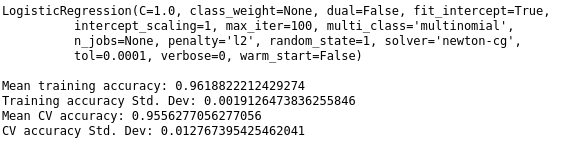
\includegraphics[scale=0.6]{img/gs-lr.png}
    \caption{Resultados de \textit{GridSearch} sobre la Regresión Logística.}
    \label{fig:gs-lr}
\end{figure}

Como podemos observar, el método ha selecciona el mismo valor para el hiperparámetro $C$ que el que nosotros habíamos prefijado en las pruebas iniciales (1.0). Este valor es el que también trae la función por defecto, y acabamos de comprobar el porque. Valores más bajos hacen que la regularización sea muy fuerte, mientras que con valores más altos el sobreajuste aparecerá debido a que los errores tendrán una mayor penalización.

Si nos paramos a analizar tanto la precisión como la desviación típica hay poco que comentar. Como los hiperparametros utilizados han sido los mismos que en las pruebas iniciales, los valores que han obtenido han sido prácticamente iguales que los anteriores, con un decimal o dos de diferencia, pero prácticamente es insignificativo.

Concluimos que, pese a no haber mejorado porque ya habíamos elegido los valores más adecuados, el modelo sigue clasificando bastante bien. No obstante, no lo seleccionaríamos como el mejor modelo, ya que los clasificadores Random Forest lo hacen mejor con una complejidad similar (e incluso las Redes Neuronales, aunque habría que estudiarlo en términos de complejidad), y aún no hemos estudiado sus hiperparámetros y si estos pueden hacer que mejore.

\subsection{Random Forest}

\newpage

% Pagina de bibliografia
\begin{thebibliography}{20}

\bibitem{bib:uci-repo}
UCI. \textit{Image segmentation}
\\\url{http://archive.ics.uci.edu/ml/datasets/image+segmentation}

\bibitem{logistic-regression}
Scikit-Learn. \textit{LogisticRegression}
\\\url{https://scikit-learn.org/stable/modules/generated/sklearn.linear_model.LogisticRegression.html}

\bibitem{svc}
Scikit-Learn. \textit{SVC}
\\\url{https://scikit-learn.org/stable/modules/generated/sklearn.svm.SVC.html#sklearn.svm.SVC}

\bibitem{random_forest}
Scikit-Learn. \textit{RandomForestClassifier}
\\\url{https://scikit-learn.org/stable/modules/generated/sklearn.ensemble.RandomForestClassifier.html#sklearn.ensemble.RandomForestClassifier}

\bibitem{neural_network}
Scikit-Learn. \textit{MLPClassifier}
\\\url{https://scikit-learn.org/stable/modules/generated/sklearn.neural_network.MLPClassifier.html#sklearn.neural_network.MLPClassifier}

\bibitem{scaler}
Scikit-Learn. \textit{StandardScaler}
\\\url{https://scikit-learn.org/stable/modules/generated/sklearn.preprocessing.StandardScaler.html}

\bibitem{pca}
Scikit-Learn. \textit{PCA}
\\\url{https://scikit-learn.org/stable/modules/generated/sklearn.decomposition.PCA.html}

\bibitem{learning_curve}
Scikit-Learn \textit{plot\_learning\_curve}
\\\url{https://scikit-learn.org/stable/auto_examples/model_selection/plot_learning_curve.html#sphx-glr-auto-examples-model-selection-plot-learning-curve-py}

\bibitem{GridSearchCV}
Scikit-Learn \textit{GridSearchCV}
\\\url{https://scikit-learn.org/stable/modules/generated/sklearn.model_selection.GridSearchCV.html}

\end{thebibliography}

\end{document}

